\documentclass[sigplan,screen]{acmart}

%% Rights management information.  This information is sent to you
%% when you complete the rights form.  These commands have SAMPLE
%% values in them; it is your responsibility as an author to replace
%% the commands and values with those provided to you when you
%% complete the rights form.
\setcopyright{acmcopyright}
\copyrightyear{2022}
\acmYear{2022}

%% These commands are for a PROCEEDINGS abstract or paper.
\acmConference{November-29-2022}{Clemson, SC}


%%
%% Submission ID.
%% Use this when submitting an article to a sponsored event. You'll
%% receive a unique submission ID from the organizers
%% of the event, and this ID should be used as the parameter to this command.
%%\acmSubmissionID{123-A56-BU3}

%%
%% For managing citations, it is recommended to use bibliography
%% files in BibTeX format.
%%
%% You can then either use BibTeX with the ACM-Reference-Format style,
%% or BibLaTeX with the acmnumeric or acmauthoryear sytles, that include
%% support for advanced citation of software artefact from the
%% biblatex-software package, also separately available on CTAN.
%%
%% Look at the sample-*-biblatex.tex files for templates showcasing
%% the biblatex styles.
%%

%%
%% The majority of ACM publications use numbered citations and
%% references.  The command \citestyle{authoryear} switches to the
%% "author year" style.
%%
%% If you are preparing content for an event
%% sponsored by ACM SIGGRAPH, you must use the "author year" style of
%% citations and references.
%% Uncommenting
%% the next command will enable that style.
%%\citestyle{acmauthoryear}

%%
%% end of the preamble, start of the body of the document source.
\begin{document}

%%
%% The "title" command has an optional parameter,
%% allowing the author to define a "short title" to be used in page headers.
\title{Snake Re-imagined in a Haunted Challenge}

%%
%% The "author" command and its associated commands are used to define
%% the authors and their affiliations.
%% Of note is the shared affiliation of the first two authors, and the
%% "authornote" and "authornotemark" commands
%% used to denote shared contribution to the research.
\author{William Sherrer}
\authornote{All authors contributed to this research.}
\email{wsherre@g.clemson.edu}
\affiliation{
  \institution{Clemson University}
  \country{Clemson, SC, USA}
}

\author{Ashton Sobeck}
\email{asobeck@g.clemson.edu}
\affiliation{
  \institution{Clemson University}
  \country{Clemson, SC, USA}
}

\author{Mohit Singh}
\email{msingh3@g.clemson.edu}
\affiliation{
  \institution{Clemson University}
  \country{Clemson, SC, USA}
}

\author{Samuel Kannan}
\email{kannan2@g.clemson.edu}
\affiliation{
  \institution{Clemson University}
  \country{Clemson, SC, USA}
}


%%
%% By default, the full list of authors will be used in the page
%% headers. Often, this list is too long, and will overlap
%% other information printed in the page headers. This command allows
%% the author to define a more concise list
%% of authors' names for this purpose.
\renewcommand{\shortauthors}{Sherrer, Sobeck, Mingh and Kannan.}
%%
%% The abstract is a short summary of the work to be presented in the
%% article.
\begin{abstract}
  For our project, we wanted to create an interactive game on more than a static template. We were tasked with creating a Halloween-styled game that is object-oriented and uses two design patterns. The game we made is Haunted Ghost Snake. It is a Halloween-themed version of the classic game Snake. Our game consists of a transparent ghost-like snake moving around to devour pumpkins. The player must navigate different levels and difficulties, allowing them to face more difficult challenges. Additionally, the player can customize the color of the snake and the game's background. The game is developed in Python 3 and uses the popular gaming package Pygame. We used 2 OOP (Object Oriented Programming) design patterns. The first is the singleton design pattern ensuring that only one instance of the game is running. We also used the clone pattern whenever a new pumpkin is made. We had fun developing this game and wish the players to have as much fun playing it.
\end{abstract}

%%
%% The code below is generated by the tool at http://dl.acm.org/ccs.cfm.
%% Please copy and paste the code instead of the example below.
%%
\begin{CCSXML}
<ccs2012>
 <concept>
  <concept_desc>Object Oriented Programming</concept_desc>
 </concept>
 <concept>
  <concept_desc></concept_desc>
 </concept>
</ccs2012>
\end{CCSXML}

\ccsdesc[500]{Object Oriented Programming}
\ccsdesc[300]{Architecture Designs~Singleton, Clone}

%%
%% Keywords. The author(s) should pick words that accurately describe
%% the work being presented. Separate the keywords with commas.
\keywords{Python, Pygame, Object Oriented Programming, Singleton, Clone}

%%
%% This command processes the author and affiliation and title
%% information and builds the first part of the formatted document.
\maketitle


\section{Introduction}
\begin{figure}[h]
  \centering
  \includegraphics[width=\linewidth]{game_home}
  \caption{Home screen of our game. }
  \Description{A screenshot of the game's home screen with buttons to change the difficulty, change the level, and adjust the settings.}
\end{figure}
The classic game Snake has been around for decades on digital devices. The game has a lot of variety and diversity in many different genres of technology. Therefore, we wanted to create our edition of this game in a Halloween format. Our game follows the traditional aspects of Snake. It starts as a tiny snake moving around, eating food, and growing until it has eaten all of the food. In this theme, we have replaced it with a "ghost" snake and the food with pumpkins. As the snake eats a pumpkin, the player can watch it travel down its length until it's fully digested. 

	We wanted to enhance the user experience while playing this game. In this game, there are a variety of different customization settings as well as different gameplay modes. The first thing we did was to create different difficulty settings that can be applied to all game modes. This is accomplished by moving the snake at different speeds on the game screen. We also added options to customize the color of the snake as well as the background image. Although all of these options increase the visual diversity of the game, we still wanted to add some actual difficulty for the player to encounter. 
	
	There is also an option on the home screen for the player to select different levels. The levels become increasingly complex as the user progresses up the rank. The player will face challenges that require them to think critically about their next move. However, where would all the fun be if they only experience static obstacles?  We wanted to create a dynamic option that changes as the player navigates their path. Thus we created a random level that changes at every start of the game. The walls also move as the game progresses to challenge the user. 
	
	At each stage of development, we discovered entertaining ways to add functionality to this game. As time went on, we added features that make this game more enjoyable for players. We made sure that this game is enjoyable long-term by adding an automatic save and restore feature. The high scores and previous settings are stored and ready to be retrieved at the next opening of the game. This game has been designed in a way where features, levels, colors, and styles can be easily added or removed to continue building off of this project.  

\section{Implementation}

There are many different implementation styles of the game "Snake." We wanted to simplify the design of our code to allow a dynamic implementation. We split the screen into blocks of pixels. Each block is 32x32 pixels big. Having the screen in a grid pattern makes for easier object placement. Three different objects can appear. They are the body of the snake, a wall that blocks the snake's path, and the pumpkin that grows the snake upon consumption. Each object is a 32x32 pixel art drawing that we created. Dividing the game into a grid allows for easier tracking of these objects. We can track each of their x and y coordinates instead of keeping track of their pixel location. To show the item on the screen, we multiply the x and y coordinates by "block\_size," which is 32 pixels. At that position, we add the image and a rectangle of size 32x32. We use the rectangle for collision detection. 

\begin{figure}[h]
  \centering
  \includegraphics[width=\linewidth]{settings}
  \caption{Settings page for game customization.}
  \Description{A screenshot of the game's settings page with options to change the snake color and background image}
\end{figure}

As shown in figure 2, the user can change the game's background and the snake's color. Changing the game background is as simple as telling Pygame which image to use. Changing the snake's color, however, is challenging. Each part of the snake body is a PNG image. Therefore to change the color, we must open each image and replace the current pixels with the new ones. Thankfully traversing images is not burdensome in Python. We store the current color in a JSON file with its RGB values. When a player wants to change the color, we open each PNG image of the snake and replace any pixel equaling the current RGB values with the new RGB color values. Then we save the image and store the new color as the current one in the JSON file. 

\subsection{Snake Implementation}

The snake is a unique aspect of the game because it moves on the screen. If we move the snake 1 pixel at a time, we run into issues when the snake turns. Other implementations of this game get around this since they use blocks for each part of the snake. We custom-designed our snake with a head, body, and tail. We can keep track of the coordinates of each part of the snake to place it on the screen. The coordinates of each part of the snake are in an iterable list. We can draw the snake by looping through this list, multiplying the x and y coordinates by the "block\_size," and placing the correct image at that location. The function that accomplishes this determines the image at that location. For example, the first and last blocks are the head and the tail. We orient the snake's head according to its direction (user input.) The function decides the rest of the body parts by the blocks in front and behind them. If the block in front of them is to the right, and the block behind them is below, then that block should be a corner piece facing right and down.

Each snake body part also has a rectangle used for collision detection. Moving the snake is very simple. We can add a coordinate in the front of the list in the direction the head is facing. Then we pop the last coordinate of the snake. If the snake ate a pumpkin, we put a coordinate at the front without deleting the tail. 

\subsection{Level Implementation}

\begin{figure}[h]
  \centering
  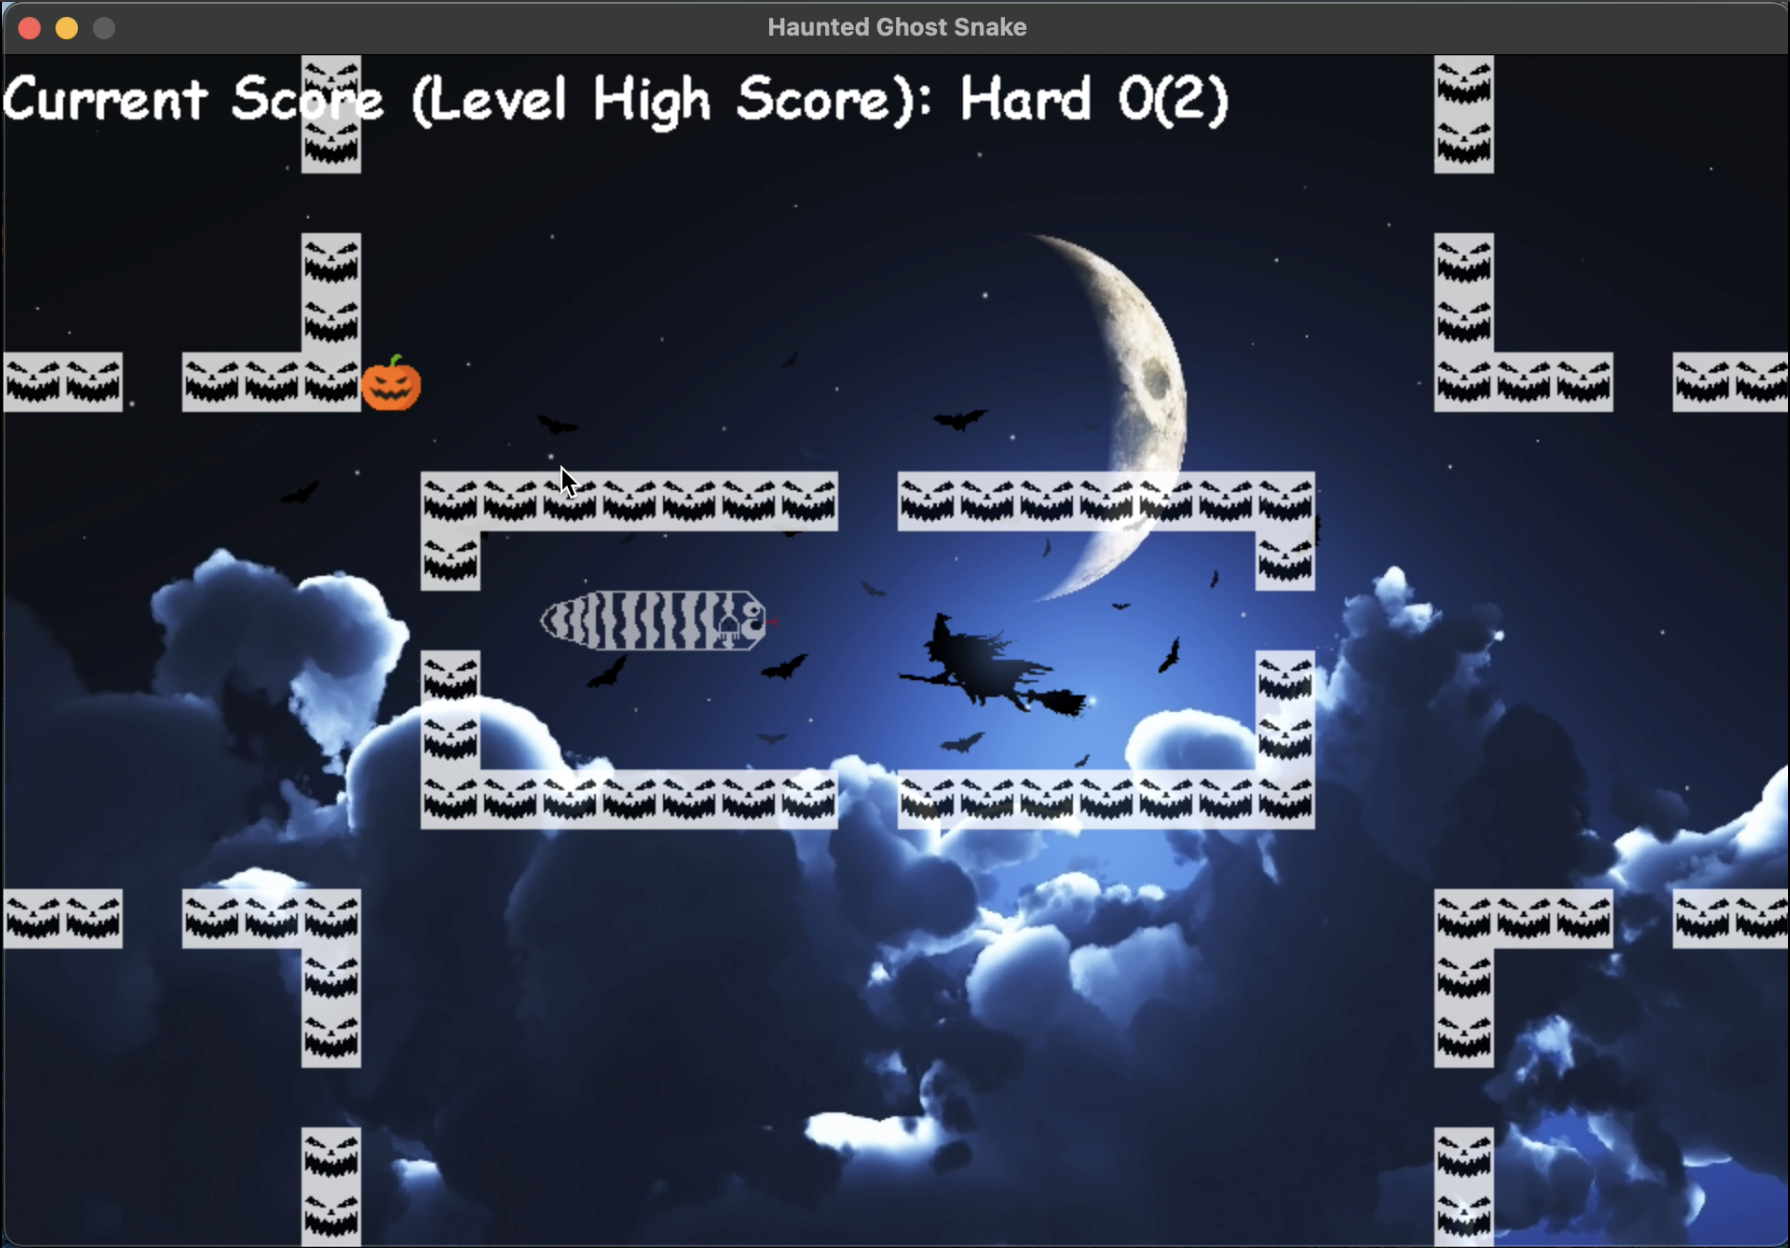
\includegraphics[width=\linewidth]{gameplay_static_level}
  \caption{Snake avoiding obstacles in one of the levels.}
  \Description{A screenshot of the gameplay with a snake moving in a level.}
\end{figure}

Levels are implemented similarly to the snake. The game stores them as a list of coordinates. This list is loaded into the game whenever a user selects a specific level. When the user starts the game, the rectangles and block images are loaded. While the game is running, the controller passes the list of rectangles to the snake. If the snake head collides with a rectangle, the game is over, and the score is displayed. 

\subsection{Random Level Implementation} 

Random levels are a subset of levels for the game. Instead of having a set position of the blockers similar to the static levels, the random level creates a random set of blockers each time the player plays the game. There are three methods that lead to the creation of random levels: a column creation method, a row creation method, and a diagonal creation method. These methods take in an x, a y, a length and a blocker. The blocker is used for the clone method so a list of blockers can be created. Currently, the creation of a random level consists of making 1-5 columns of length 1 to 5 blocks, 1 to 5 rows of length 1 to 5 blocks and 1 to 5 diagonals of length 1 to 5 blocks. All of these structures are randomly placed in order to create the random level. This allows for a very replayable experience for the player in order to have a unique level each time they play the game.

\subsection{Pumpkin Implementation}

The final object that we must render is the pumpkin. This object is different since we must keep track of each pumpkin. The game controller handles this task by keeping a list of each pumpkin instance. We wanted to add a Halloween-themed aspect to our pumpkin. Each time the snake eats the pumpkin, the player can watch it travel through the snake. We accomplished this by "disabling" the pumpkin once the snake ate it (collided with the head.) We then make the pumpkin 50\% transparent to give the illusion that it's in the snake. Since each snake's body part follows the part in front of it, we can guarantee it will traverse the whole snake. We change how we handle a disabled pumpkin. Since the pumpkin is traversing the snake, we check for when they are not colliding. Once they stop, we can delete this pumpkin from the list. 

\subsection{Design Patterns}
We implement two design patterns in our game. The first pattern is the Singleton design pattern. It's the driver of the game that ensures there is only one instance. The Singleton class has one method that houses the controller and variables required for the game to function. The second pattern we use is the clone pattern. Each time the snake eats a pumpkin, the controller requests a clone of the pumpkin. Then this new pumpkin is placed in a random position in the game, not in the snake or walls. 

We implemented our game using Pygame \cite{pygame}. Pygame includes a GUI along with other libraries that streamline game development. Our game updates the screen 60 times per second. Since we are using a grid, we set a timer to control the snake's movement. When the timer hits zero, we move the snake in the direction it's facing, then reset it. We adjust the difficulty of the game by changing this timer. The smaller the time, the more often the snake is moved. Therefore, the player perceives the snake as moving faster and vice versa.

\section{Challenges}
The development of this game presented several challenges. First, we had to figure out how to move the snake. You can do this by adding or subtracting its x and y coordinates. However, this is challenging since the corners won't match the body. We solved this problem by implementing a grid. We can move each part of the snake along the grid, which is easier to implement. As the code expanded, we realized that we weren't doing an efficient job of encapsulation. To overcome this, we added a class called "Screens" that manages the screens displayed and the objects on those screens. The driver function in the Singleton class takes control when the player starts the game. It's also responsible for resetting the game when the player's snake dies. We faced a challenge with keeping track of the objects on the screen. We realized the easiest solution was for each class to have a list of coordinates for placement and a list of rectangles for collisions. Then after we move the snake, we can pass the list of rectangles, along with the pumpkin, to the snake so that it can check for a collision. 

\section{Conclusion}
Our goal was to create a Halloween-themed game with different customizable options and challenges for the player. We believe that we met our expectations and exceeded them. This game represents a project that allowed us to put different software design patterns into practice. Utilizing these different design patterns expands our knowledge and further prepares us for entering the software engineering field. We implemented the game in a manner that allows for additional growth. We hope this project can inspire future students to continue developing projects that bring them joy.\cite{code} 

\bibliographystyle{ACM-Reference-Format}
\bibliography{refs}

\end{document}

